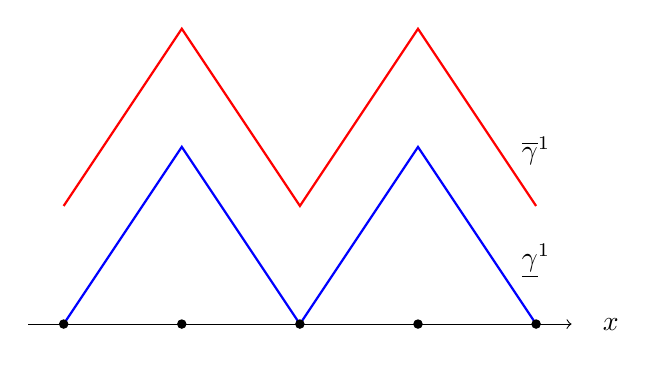
\begin{tikzpicture}[scale=1.5]
  \draw[blue,thick] (0.0,0.0) -- (1.0,1.5) -- (2.0,0.0) -- (3.0,1.5) -- (4.0,0.0)
                     node [yshift=8mm] {{\color{black} $\underline{\gamma}^1$}};
  \draw[red,thick] (0.0,1.0) -- (1.0,2.5) -- (2.0,1.0) -- (3.0,2.5) -- (4.0,1.0)
                     node [yshift=7mm] {{\color{black} $\overline{\gamma}^1$}};
  \draw[black,thin,->] (-0.3,0.0) -- (4.3,0.0) node [xshift=5mm] {$x$};
  \foreach \x in {0.0, 1.0, 2.0, 3.0, 4.0} {
      \filldraw (\x,0.0) circle (1.0pt);
  }
\end{tikzpicture}
